
% Default to the notebook output style

    


% Inherit from the specified cell style.




    
\documentclass[11pt]{article}

    
    
    \usepackage[T1]{fontenc}
    % Nicer default font (+ math font) than Computer Modern for most use cases
    \usepackage{mathpazo}

    % Basic figure setup, for now with no caption control since it's done
    % automatically by Pandoc (which extracts ![](path) syntax from Markdown).
    \usepackage{graphicx}
    % We will generate all images so they have a width \maxwidth. This means
    % that they will get their normal width if they fit onto the page, but
    % are scaled down if they would overflow the margins.
    \makeatletter
    \def\maxwidth{\ifdim\Gin@nat@width>\linewidth\linewidth
    \else\Gin@nat@width\fi}
    \makeatother
    \let\Oldincludegraphics\includegraphics
    % Set max figure width to be 80% of text width, for now hardcoded.
    \renewcommand{\includegraphics}[1]{\Oldincludegraphics[width=.8\maxwidth]{#1}}
    % Ensure that by default, figures have no caption (until we provide a
    % proper Figure object with a Caption API and a way to capture that
    % in the conversion process - todo).
    \usepackage{caption}
    \DeclareCaptionLabelFormat{nolabel}{}
    \captionsetup{labelformat=nolabel}

    \usepackage{adjustbox} % Used to constrain images to a maximum size 
    \usepackage{xcolor} % Allow colors to be defined
    \usepackage{enumerate} % Needed for markdown enumerations to work
    \usepackage{geometry} % Used to adjust the document margins
    \usepackage{amsmath} % Equations
    \usepackage{amssymb} % Equations
    \usepackage{textcomp} % defines textquotesingle
    % Hack from http://tex.stackexchange.com/a/47451/13684:
    \AtBeginDocument{%
        \def\PYZsq{\textquotesingle}% Upright quotes in Pygmentized code
    }
    \usepackage{upquote} % Upright quotes for verbatim code
    \usepackage{eurosym} % defines \euro
    \usepackage[mathletters]{ucs} % Extended unicode (utf-8) support
    \usepackage[utf8x]{inputenc} % Allow utf-8 characters in the tex document
    \usepackage{fancyvrb} % verbatim replacement that allows latex
    \usepackage{grffile} % extends the file name processing of package graphics 
                         % to support a larger range 
    % The hyperref package gives us a pdf with properly built
    % internal navigation ('pdf bookmarks' for the table of contents,
    % internal cross-reference links, web links for URLs, etc.)
    \usepackage{hyperref}
    \usepackage{longtable} % longtable support required by pandoc >1.10
    \usepackage{booktabs}  % table support for pandoc > 1.12.2
    \usepackage[inline]{enumitem} % IRkernel/repr support (it uses the enumerate* environment)
    \usepackage[normalem]{ulem} % ulem is needed to support strikethroughs (\sout)
                                % normalem makes italics be italics, not underlines
    

    
    
    % Colors for the hyperref package
    \definecolor{urlcolor}{rgb}{0,.145,.698}
    \definecolor{linkcolor}{rgb}{.71,0.21,0.01}
    \definecolor{citecolor}{rgb}{.12,.54,.11}

    % ANSI colors
    \definecolor{ansi-black}{HTML}{3E424D}
    \definecolor{ansi-black-intense}{HTML}{282C36}
    \definecolor{ansi-red}{HTML}{E75C58}
    \definecolor{ansi-red-intense}{HTML}{B22B31}
    \definecolor{ansi-green}{HTML}{00A250}
    \definecolor{ansi-green-intense}{HTML}{007427}
    \definecolor{ansi-yellow}{HTML}{DDB62B}
    \definecolor{ansi-yellow-intense}{HTML}{B27D12}
    \definecolor{ansi-blue}{HTML}{208FFB}
    \definecolor{ansi-blue-intense}{HTML}{0065CA}
    \definecolor{ansi-magenta}{HTML}{D160C4}
    \definecolor{ansi-magenta-intense}{HTML}{A03196}
    \definecolor{ansi-cyan}{HTML}{60C6C8}
    \definecolor{ansi-cyan-intense}{HTML}{258F8F}
    \definecolor{ansi-white}{HTML}{C5C1B4}
    \definecolor{ansi-white-intense}{HTML}{A1A6B2}

    % commands and environments needed by pandoc snippets
    % extracted from the output of `pandoc -s`
    \providecommand{\tightlist}{%
      \setlength{\itemsep}{0pt}\setlength{\parskip}{0pt}}
    \DefineVerbatimEnvironment{Highlighting}{Verbatim}{commandchars=\\\{\}}
    % Add ',fontsize=\small' for more characters per line
    \newenvironment{Shaded}{}{}
    \newcommand{\KeywordTok}[1]{\textcolor[rgb]{0.00,0.44,0.13}{\textbf{{#1}}}}
    \newcommand{\DataTypeTok}[1]{\textcolor[rgb]{0.56,0.13,0.00}{{#1}}}
    \newcommand{\DecValTok}[1]{\textcolor[rgb]{0.25,0.63,0.44}{{#1}}}
    \newcommand{\BaseNTok}[1]{\textcolor[rgb]{0.25,0.63,0.44}{{#1}}}
    \newcommand{\FloatTok}[1]{\textcolor[rgb]{0.25,0.63,0.44}{{#1}}}
    \newcommand{\CharTok}[1]{\textcolor[rgb]{0.25,0.44,0.63}{{#1}}}
    \newcommand{\StringTok}[1]{\textcolor[rgb]{0.25,0.44,0.63}{{#1}}}
    \newcommand{\CommentTok}[1]{\textcolor[rgb]{0.38,0.63,0.69}{\textit{{#1}}}}
    \newcommand{\OtherTok}[1]{\textcolor[rgb]{0.00,0.44,0.13}{{#1}}}
    \newcommand{\AlertTok}[1]{\textcolor[rgb]{1.00,0.00,0.00}{\textbf{{#1}}}}
    \newcommand{\FunctionTok}[1]{\textcolor[rgb]{0.02,0.16,0.49}{{#1}}}
    \newcommand{\RegionMarkerTok}[1]{{#1}}
    \newcommand{\ErrorTok}[1]{\textcolor[rgb]{1.00,0.00,0.00}{\textbf{{#1}}}}
    \newcommand{\NormalTok}[1]{{#1}}
    
    % Additional commands for more recent versions of Pandoc
    \newcommand{\ConstantTok}[1]{\textcolor[rgb]{0.53,0.00,0.00}{{#1}}}
    \newcommand{\SpecialCharTok}[1]{\textcolor[rgb]{0.25,0.44,0.63}{{#1}}}
    \newcommand{\VerbatimStringTok}[1]{\textcolor[rgb]{0.25,0.44,0.63}{{#1}}}
    \newcommand{\SpecialStringTok}[1]{\textcolor[rgb]{0.73,0.40,0.53}{{#1}}}
    \newcommand{\ImportTok}[1]{{#1}}
    \newcommand{\DocumentationTok}[1]{\textcolor[rgb]{0.73,0.13,0.13}{\textit{{#1}}}}
    \newcommand{\AnnotationTok}[1]{\textcolor[rgb]{0.38,0.63,0.69}{\textbf{\textit{{#1}}}}}
    \newcommand{\CommentVarTok}[1]{\textcolor[rgb]{0.38,0.63,0.69}{\textbf{\textit{{#1}}}}}
    \newcommand{\VariableTok}[1]{\textcolor[rgb]{0.10,0.09,0.49}{{#1}}}
    \newcommand{\ControlFlowTok}[1]{\textcolor[rgb]{0.00,0.44,0.13}{\textbf{{#1}}}}
    \newcommand{\OperatorTok}[1]{\textcolor[rgb]{0.40,0.40,0.40}{{#1}}}
    \newcommand{\BuiltInTok}[1]{{#1}}
    \newcommand{\ExtensionTok}[1]{{#1}}
    \newcommand{\PreprocessorTok}[1]{\textcolor[rgb]{0.74,0.48,0.00}{{#1}}}
    \newcommand{\AttributeTok}[1]{\textcolor[rgb]{0.49,0.56,0.16}{{#1}}}
    \newcommand{\InformationTok}[1]{\textcolor[rgb]{0.38,0.63,0.69}{\textbf{\textit{{#1}}}}}
    \newcommand{\WarningTok}[1]{\textcolor[rgb]{0.38,0.63,0.69}{\textbf{\textit{{#1}}}}}
    
    
    % Define a nice break command that doesn't care if a line doesn't already
    % exist.
    \def\br{\hspace*{\fill} \\* }
    % Math Jax compatability definitions
    \def\gt{>}
    \def\lt{<}
    % Document parameters
    \title{slides\_djelfa2018}
    
    
    

    % Pygments definitions
    
\makeatletter
\def\PY@reset{\let\PY@it=\relax \let\PY@bf=\relax%
    \let\PY@ul=\relax \let\PY@tc=\relax%
    \let\PY@bc=\relax \let\PY@ff=\relax}
\def\PY@tok#1{\csname PY@tok@#1\endcsname}
\def\PY@toks#1+{\ifx\relax#1\empty\else%
    \PY@tok{#1}\expandafter\PY@toks\fi}
\def\PY@do#1{\PY@bc{\PY@tc{\PY@ul{%
    \PY@it{\PY@bf{\PY@ff{#1}}}}}}}
\def\PY#1#2{\PY@reset\PY@toks#1+\relax+\PY@do{#2}}

\expandafter\def\csname PY@tok@w\endcsname{\def\PY@tc##1{\textcolor[rgb]{0.73,0.73,0.73}{##1}}}
\expandafter\def\csname PY@tok@c\endcsname{\let\PY@it=\textit\def\PY@tc##1{\textcolor[rgb]{0.25,0.50,0.50}{##1}}}
\expandafter\def\csname PY@tok@cp\endcsname{\def\PY@tc##1{\textcolor[rgb]{0.74,0.48,0.00}{##1}}}
\expandafter\def\csname PY@tok@k\endcsname{\let\PY@bf=\textbf\def\PY@tc##1{\textcolor[rgb]{0.00,0.50,0.00}{##1}}}
\expandafter\def\csname PY@tok@kp\endcsname{\def\PY@tc##1{\textcolor[rgb]{0.00,0.50,0.00}{##1}}}
\expandafter\def\csname PY@tok@kt\endcsname{\def\PY@tc##1{\textcolor[rgb]{0.69,0.00,0.25}{##1}}}
\expandafter\def\csname PY@tok@o\endcsname{\def\PY@tc##1{\textcolor[rgb]{0.40,0.40,0.40}{##1}}}
\expandafter\def\csname PY@tok@ow\endcsname{\let\PY@bf=\textbf\def\PY@tc##1{\textcolor[rgb]{0.67,0.13,1.00}{##1}}}
\expandafter\def\csname PY@tok@nb\endcsname{\def\PY@tc##1{\textcolor[rgb]{0.00,0.50,0.00}{##1}}}
\expandafter\def\csname PY@tok@nf\endcsname{\def\PY@tc##1{\textcolor[rgb]{0.00,0.00,1.00}{##1}}}
\expandafter\def\csname PY@tok@nc\endcsname{\let\PY@bf=\textbf\def\PY@tc##1{\textcolor[rgb]{0.00,0.00,1.00}{##1}}}
\expandafter\def\csname PY@tok@nn\endcsname{\let\PY@bf=\textbf\def\PY@tc##1{\textcolor[rgb]{0.00,0.00,1.00}{##1}}}
\expandafter\def\csname PY@tok@ne\endcsname{\let\PY@bf=\textbf\def\PY@tc##1{\textcolor[rgb]{0.82,0.25,0.23}{##1}}}
\expandafter\def\csname PY@tok@nv\endcsname{\def\PY@tc##1{\textcolor[rgb]{0.10,0.09,0.49}{##1}}}
\expandafter\def\csname PY@tok@no\endcsname{\def\PY@tc##1{\textcolor[rgb]{0.53,0.00,0.00}{##1}}}
\expandafter\def\csname PY@tok@nl\endcsname{\def\PY@tc##1{\textcolor[rgb]{0.63,0.63,0.00}{##1}}}
\expandafter\def\csname PY@tok@ni\endcsname{\let\PY@bf=\textbf\def\PY@tc##1{\textcolor[rgb]{0.60,0.60,0.60}{##1}}}
\expandafter\def\csname PY@tok@na\endcsname{\def\PY@tc##1{\textcolor[rgb]{0.49,0.56,0.16}{##1}}}
\expandafter\def\csname PY@tok@nt\endcsname{\let\PY@bf=\textbf\def\PY@tc##1{\textcolor[rgb]{0.00,0.50,0.00}{##1}}}
\expandafter\def\csname PY@tok@nd\endcsname{\def\PY@tc##1{\textcolor[rgb]{0.67,0.13,1.00}{##1}}}
\expandafter\def\csname PY@tok@s\endcsname{\def\PY@tc##1{\textcolor[rgb]{0.73,0.13,0.13}{##1}}}
\expandafter\def\csname PY@tok@sd\endcsname{\let\PY@it=\textit\def\PY@tc##1{\textcolor[rgb]{0.73,0.13,0.13}{##1}}}
\expandafter\def\csname PY@tok@si\endcsname{\let\PY@bf=\textbf\def\PY@tc##1{\textcolor[rgb]{0.73,0.40,0.53}{##1}}}
\expandafter\def\csname PY@tok@se\endcsname{\let\PY@bf=\textbf\def\PY@tc##1{\textcolor[rgb]{0.73,0.40,0.13}{##1}}}
\expandafter\def\csname PY@tok@sr\endcsname{\def\PY@tc##1{\textcolor[rgb]{0.73,0.40,0.53}{##1}}}
\expandafter\def\csname PY@tok@ss\endcsname{\def\PY@tc##1{\textcolor[rgb]{0.10,0.09,0.49}{##1}}}
\expandafter\def\csname PY@tok@sx\endcsname{\def\PY@tc##1{\textcolor[rgb]{0.00,0.50,0.00}{##1}}}
\expandafter\def\csname PY@tok@m\endcsname{\def\PY@tc##1{\textcolor[rgb]{0.40,0.40,0.40}{##1}}}
\expandafter\def\csname PY@tok@gh\endcsname{\let\PY@bf=\textbf\def\PY@tc##1{\textcolor[rgb]{0.00,0.00,0.50}{##1}}}
\expandafter\def\csname PY@tok@gu\endcsname{\let\PY@bf=\textbf\def\PY@tc##1{\textcolor[rgb]{0.50,0.00,0.50}{##1}}}
\expandafter\def\csname PY@tok@gd\endcsname{\def\PY@tc##1{\textcolor[rgb]{0.63,0.00,0.00}{##1}}}
\expandafter\def\csname PY@tok@gi\endcsname{\def\PY@tc##1{\textcolor[rgb]{0.00,0.63,0.00}{##1}}}
\expandafter\def\csname PY@tok@gr\endcsname{\def\PY@tc##1{\textcolor[rgb]{1.00,0.00,0.00}{##1}}}
\expandafter\def\csname PY@tok@ge\endcsname{\let\PY@it=\textit}
\expandafter\def\csname PY@tok@gs\endcsname{\let\PY@bf=\textbf}
\expandafter\def\csname PY@tok@gp\endcsname{\let\PY@bf=\textbf\def\PY@tc##1{\textcolor[rgb]{0.00,0.00,0.50}{##1}}}
\expandafter\def\csname PY@tok@go\endcsname{\def\PY@tc##1{\textcolor[rgb]{0.53,0.53,0.53}{##1}}}
\expandafter\def\csname PY@tok@gt\endcsname{\def\PY@tc##1{\textcolor[rgb]{0.00,0.27,0.87}{##1}}}
\expandafter\def\csname PY@tok@err\endcsname{\def\PY@bc##1{\setlength{\fboxsep}{0pt}\fcolorbox[rgb]{1.00,0.00,0.00}{1,1,1}{\strut ##1}}}
\expandafter\def\csname PY@tok@kc\endcsname{\let\PY@bf=\textbf\def\PY@tc##1{\textcolor[rgb]{0.00,0.50,0.00}{##1}}}
\expandafter\def\csname PY@tok@kd\endcsname{\let\PY@bf=\textbf\def\PY@tc##1{\textcolor[rgb]{0.00,0.50,0.00}{##1}}}
\expandafter\def\csname PY@tok@kn\endcsname{\let\PY@bf=\textbf\def\PY@tc##1{\textcolor[rgb]{0.00,0.50,0.00}{##1}}}
\expandafter\def\csname PY@tok@kr\endcsname{\let\PY@bf=\textbf\def\PY@tc##1{\textcolor[rgb]{0.00,0.50,0.00}{##1}}}
\expandafter\def\csname PY@tok@bp\endcsname{\def\PY@tc##1{\textcolor[rgb]{0.00,0.50,0.00}{##1}}}
\expandafter\def\csname PY@tok@fm\endcsname{\def\PY@tc##1{\textcolor[rgb]{0.00,0.00,1.00}{##1}}}
\expandafter\def\csname PY@tok@vc\endcsname{\def\PY@tc##1{\textcolor[rgb]{0.10,0.09,0.49}{##1}}}
\expandafter\def\csname PY@tok@vg\endcsname{\def\PY@tc##1{\textcolor[rgb]{0.10,0.09,0.49}{##1}}}
\expandafter\def\csname PY@tok@vi\endcsname{\def\PY@tc##1{\textcolor[rgb]{0.10,0.09,0.49}{##1}}}
\expandafter\def\csname PY@tok@vm\endcsname{\def\PY@tc##1{\textcolor[rgb]{0.10,0.09,0.49}{##1}}}
\expandafter\def\csname PY@tok@sa\endcsname{\def\PY@tc##1{\textcolor[rgb]{0.73,0.13,0.13}{##1}}}
\expandafter\def\csname PY@tok@sb\endcsname{\def\PY@tc##1{\textcolor[rgb]{0.73,0.13,0.13}{##1}}}
\expandafter\def\csname PY@tok@sc\endcsname{\def\PY@tc##1{\textcolor[rgb]{0.73,0.13,0.13}{##1}}}
\expandafter\def\csname PY@tok@dl\endcsname{\def\PY@tc##1{\textcolor[rgb]{0.73,0.13,0.13}{##1}}}
\expandafter\def\csname PY@tok@s2\endcsname{\def\PY@tc##1{\textcolor[rgb]{0.73,0.13,0.13}{##1}}}
\expandafter\def\csname PY@tok@sh\endcsname{\def\PY@tc##1{\textcolor[rgb]{0.73,0.13,0.13}{##1}}}
\expandafter\def\csname PY@tok@s1\endcsname{\def\PY@tc##1{\textcolor[rgb]{0.73,0.13,0.13}{##1}}}
\expandafter\def\csname PY@tok@mb\endcsname{\def\PY@tc##1{\textcolor[rgb]{0.40,0.40,0.40}{##1}}}
\expandafter\def\csname PY@tok@mf\endcsname{\def\PY@tc##1{\textcolor[rgb]{0.40,0.40,0.40}{##1}}}
\expandafter\def\csname PY@tok@mh\endcsname{\def\PY@tc##1{\textcolor[rgb]{0.40,0.40,0.40}{##1}}}
\expandafter\def\csname PY@tok@mi\endcsname{\def\PY@tc##1{\textcolor[rgb]{0.40,0.40,0.40}{##1}}}
\expandafter\def\csname PY@tok@il\endcsname{\def\PY@tc##1{\textcolor[rgb]{0.40,0.40,0.40}{##1}}}
\expandafter\def\csname PY@tok@mo\endcsname{\def\PY@tc##1{\textcolor[rgb]{0.40,0.40,0.40}{##1}}}
\expandafter\def\csname PY@tok@ch\endcsname{\let\PY@it=\textit\def\PY@tc##1{\textcolor[rgb]{0.25,0.50,0.50}{##1}}}
\expandafter\def\csname PY@tok@cm\endcsname{\let\PY@it=\textit\def\PY@tc##1{\textcolor[rgb]{0.25,0.50,0.50}{##1}}}
\expandafter\def\csname PY@tok@cpf\endcsname{\let\PY@it=\textit\def\PY@tc##1{\textcolor[rgb]{0.25,0.50,0.50}{##1}}}
\expandafter\def\csname PY@tok@c1\endcsname{\let\PY@it=\textit\def\PY@tc##1{\textcolor[rgb]{0.25,0.50,0.50}{##1}}}
\expandafter\def\csname PY@tok@cs\endcsname{\let\PY@it=\textit\def\PY@tc##1{\textcolor[rgb]{0.25,0.50,0.50}{##1}}}

\def\PYZbs{\char`\\}
\def\PYZus{\char`\_}
\def\PYZob{\char`\{}
\def\PYZcb{\char`\}}
\def\PYZca{\char`\^}
\def\PYZam{\char`\&}
\def\PYZlt{\char`\<}
\def\PYZgt{\char`\>}
\def\PYZsh{\char`\#}
\def\PYZpc{\char`\%}
\def\PYZdl{\char`\$}
\def\PYZhy{\char`\-}
\def\PYZsq{\char`\'}
\def\PYZdq{\char`\"}
\def\PYZti{\char`\~}
% for compatibility with earlier versions
\def\PYZat{@}
\def\PYZlb{[}
\def\PYZrb{]}
\makeatother


    % Exact colors from NB
    \definecolor{incolor}{rgb}{0.0, 0.0, 0.5}
    \definecolor{outcolor}{rgb}{0.545, 0.0, 0.0}



    
    % Prevent overflowing lines due to hard-to-break entities
    \sloppy 
    % Setup hyperref package
    \hypersetup{
      breaklinks=true,  % so long urls are correctly broken across lines
      colorlinks=true,
      urlcolor=urlcolor,
      linkcolor=linkcolor,
      citecolor=citecolor,
      }
    % Slightly bigger margins than the latex defaults
    
    \geometry{verbose,tmargin=1in,bmargin=1in,lmargin=1in,rmargin=1in}
    
    

    \begin{document}
    
    
    \maketitle
    
    

    
    \#

Premier pas avec IPython et Jupyter deux couteaux suisse du développeur

K.I.A.Derouiche

Mars 24, 2018 Free Djelfa

Djelfa, Algerie

    \subsection{About me}\label{about-me}

\begin{itemize}
\tightlist
\item
  Architect R\&D at ADGON Solutions
\item
  Membre de l'association A2DMETI
\item
  \href{http://github.com/kiaderouiche}{GitHub}
\end{itemize}

\paragraph{Contact}\label{contact}

\begin{itemize}
\tightlist
\item
  {[}@kiaderouiche{]}(http://twitter.com/kiaderouiche)
\item
  \href{mailto:kamel.derouiche@gmail.com}{Email}
\end{itemize}

    \subsection{Qui utilisent Jupyter}\label{qui-utilisent-jupyter}

\begin{figure}
\centering

\includegraphics{images/jupyter-a-platform-use.jpg}
\caption{Qui utilisent Jupyter}
\end{figure}

    \section{Introduction à IPython}\label{introduction-uxe0-ipython}

\begin{figure}
\centering

\includegraphics{images/ipython.png}
\caption{Qui utilisent Jupyter}
\end{figure}

    \section{Le commencement !}\label{le-commencement}

créé par F Perez(Photo) (chercheur au Berkeley Institute for Data
Science) en 2001.

\begin{figure}
\centering
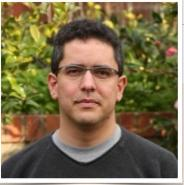
\includegraphics{images/perez.jpg}
\caption{Qui utilisent Jupyter}
\end{figure}

    \section{L'installation d'IPython, jupyter et
jupyterlab}\label{linstallation-dipython-jupyter-et-jupyterlab}

Trois méthodes d'installations:

\begin{itemize}
\tightlist
\item
  installation de paquets via les distributions.
\item
  Utilisation de l'environement virtualenv via pip:
\item
  \$ pip install -\/-user virtualenv
\item
  \$ virtualenv /path/vers/projet/env\_nom\_du\_projet
\item
  \$ source /path/vers/projet/env\_nom\_du\_projet/bin/activate
\item
  \url{https://www.anaconda.com/} : Anaconda est une distribution open
  source pour des programmation Python et R permet de faire du
  traitement de données à grande échelle, l'analyse prédictive et
  l'informatique scientifique, visant à simplifier la gestion et le
  déploiement des paquets scientifique Python gérées par le système de
  gestion de paquets conda. un seul installeur pour tous les paquets
  Python scientifique,
\end{itemize}

    \section{Au commencement il eut
IPython...}\label{au-commencement-il-eut-ipython...}

IPython un shell python évolué:

\begin{itemize}
\tightlist
\item
  coloration syntaxique
\item
  autocompletation
\item
  historiques des saisies et des résultats
\item
  commandes systèmes
\item
  aide en ligne
\item
  commandes utiles propres (\%magics)
\item
  intégration à la boucle d'évènement de divers toolkits graphiques(qt,
  gtk, wx)
\item
  pylab
\end{itemize}

    \subsection{Edition et évaluation de code
python}\label{edition-et-uxe9valuation-de-code-python}

Avec complétation automatique et coloration syntaxique.

IPython affiche le résultat de la derniére expression évaluée si elle ne
vaut pas None

    \subsection{Les fonctions magiques et propres à
IPython}\label{les-fonctions-magiques-et-propres-uxe0-ipython}

\begin{itemize}
\tightlist
\item
  commence avec \% et \%\%
\item
  \%quickref pour avoir tout les commandes
\item
  \%lsmagic lister tous les commandes magiques
\end{itemize}

Available line magics: \%alias \%alias\_magic \%autocall \%autoindent
\%automagic \%bookmark \%cat \%cd \%clear \%colors \%config \%cp
\%cpaste \%debug \%dhist \%dirs \%doctest\_mode \%ed \%edit \%env \%gui
\%hist \%history \%killbgscripts \%ldir \%less \%lf \%lk \%ll \%load
\%load\_ext \%loadpy \%logoff \%logon \%logstart \%logstate \%logstop
\%ls \%lsmagic \%lx \%macro \%magic \%man \%matplotlib \%mkdir \%more
\%mv \%notebook \%page \%paste \%pastebin \%pdb \%pdef \%pdoc \%pfile
\%pinfo \%pinfo2 \%popd \%pprint \%precision \%profile \%prun \%psearch
\%psource \%pushd \%pwd \%pycat \%pylab \%quickref \%recall \%rehashx
\%reload\_ext \%rep \%rerun \%reset \%reset\_selective \%rm \%rmdir
\%run \%save \%sc \%set\_env \%store \%sx \%system \%tb \%time \%timeit
\%unalias \%unload\_ext \%who \%who\_ls \%whos \%xdel \%xmode

Available cell magics: \%\%! \%\%HTML \%\%SVG \%\%bash \%\%capture
\%\%debug \%\%file \%\%html \%\%javascript \%\%js \%\%latex \%\%markdown
\%\%perl \%\%prun \%\%pypy \%\%python \%\%python2 \%\%python3 \%\%ruby
\%\%script \%\%sh \%\%svg \%\%sx \%\%system \%\%time \%\%timeit
\%\%writefile

Automagic is ON, \% prefix IS NOT needed for line magics.

    En lançant la commande IPython on travaille directement avec IPython,
via stdin, stdout et stderr

Outer l'économie de ressources, cela permet de l'utiliser comme un shell
systéme

    \subsection{Session IPython}\label{session-ipython}

    \begin{Verbatim}[commandchars=\\\{\}]
{\color{incolor}In [{\color{incolor} }]:} \PY{c+c1}{\PYZsh{} Demarrer le logging de la session}
        \PY{o}{\PYZpc{}}\PY{k}{logstart}
\end{Verbatim}


    \begin{Verbatim}[commandchars=\\\{\}]
{\color{incolor}In [{\color{incolor} }]:} \PY{c+c1}{\PYZsh{}Etat de la session}
        \PY{o}{\PYZpc{}}\PY{k}{logstate}
\end{Verbatim}


    \begin{Verbatim}[commandchars=\\\{\}]
{\color{incolor}In [{\color{incolor}1}]:} \PY{c+c1}{\PYZsh{}Stoppé une session}
        \PY{o}{\PYZpc{}}\PY{k}{logoff}
\end{Verbatim}


    \begin{Verbatim}[commandchars=\\\{\}]

Logging hasn't been started yet (use logstart for that).

\%logon/\%logoff are for temporarily starting and stopping logging for a logfile
which already exists. But you must first start the logging process with
\%logstart (optionally giving a logfile name).

    \end{Verbatim}

    \begin{Verbatim}[commandchars=\\\{\}]
{\color{incolor}In [{\color{incolor} }]:} \PY{c+c1}{\PYZsh{} Historique de la session}
        \PY{o}{\PYZpc{}}\PY{k}{history} \PYZsh{}or \PYZpc{}hist
\end{Verbatim}


    \begin{Verbatim}[commandchars=\\\{\}]
{\color{incolor}In [{\color{incolor}9}]:} \PY{c+c1}{\PYZsh{} Mesurer le temps d\PYZsq{}exécution}
        \PY{n}{S} \PY{o}{=} \PY{p}{[}\PY{n}{x}\PY{o}{*}\PY{o}{*}\PY{l+m+mi}{2} \PY{k}{for} \PY{n}{x} \PY{o+ow}{in} \PY{n+nb}{range}\PY{p}{(}\PY{l+m+mi}{10}\PY{p}{)}\PY{p}{]}
        \PY{o}{\PYZpc{}}\PY{k}{timeit} M = [x for x in S if x \PYZpc{} 2 == 0]
\end{Verbatim}


    \begin{Verbatim}[commandchars=\\\{\}]
891 ns ± 31.1 ns per loop (mean ± std. dev. of 7 runs, 1000000 loops each)

    \end{Verbatim}

    \subsubsection{Exécution de commandes du
shell}\label{exuxe9cution-de-commandes-du-shell}

La commande shell commence par un point d'exclamation. Est la ligne est
passé au shell du système

    \begin{Verbatim}[commandchars=\\\{\}]
{\color{incolor}In [{\color{incolor} }]:} \PY{c+c1}{\PYZsh{} avec la commande **!**}
        \PY{n}{In} \PY{p}{[}\PY{l+m+mi}{3}\PY{p}{]}\PY{p}{:} \PY{o}{!} du \PYZhy{}h /etc
\end{Verbatim}


    \subsubsection{Documentation en ligne}\label{documentation-en-ligne}

IPython propose une alternative commode à la commande help() de python
avec la syntaxe ? On peut même consulter le code source (si présent)
avec ??

    \begin{Verbatim}[commandchars=\\\{\}]
{\color{incolor}In [{\color{incolor}11}]:} \PY{k+kn}{import} \PY{n+nn}{io}
         io.BytesIO\PY{o}{?}
\end{Verbatim}


    
    \begin{verbatim}
Init signature: io.BytesIO(initial_bytes=b'')
Docstring:      Buffered I/O implementation using an in-memory bytes buffer.
Type:           type

    \end{verbatim}

    
    \begin{Verbatim}[commandchars=\\\{\}]
{\color{incolor}In [{\color{incolor}2}]:} \PY{c+c1}{\PYZsh{}\PYZsh{} Je souhaite calculer pour la valeur x = 2.0 avec SymPy et NumPy}
        \PY{k+kn}{from} \PY{n+nn}{IPython}\PY{n+nn}{.}\PY{n+nn}{display} \PY{k}{import} \PY{n}{display}\PY{p}{,} \PY{n}{Math}\PY{p}{,} \PY{n}{Latex}
        \PY{n}{display}\PY{p}{(}\PY{n}{Math}\PY{p}{(}\PY{l+s+sa}{r}\PY{l+s+s1}{\PYZsq{}}\PY{l+s+s1}{y = }\PY{l+s+s1}{\PYZbs{}}\PY{l+s+s1}{sqrt}\PY{l+s+s1}{\PYZob{}}\PY{l+s+s1}{log(1+x\PYZca{}}\PY{l+s+si}{\PYZob{}2\PYZcb{}}\PY{l+s+s1}{)+}\PY{l+s+s1}{\PYZbs{}}\PY{l+s+s1}{frac}\PY{l+s+s1}{\PYZob{}}\PY{l+s+s1}{x\PYZca{}}\PY{l+s+s1}{\PYZob{}}\PY{l+s+s1}{\PYZbs{}}\PY{l+s+s1}{sin(2}\PY{l+s+s1}{\PYZbs{}}\PY{l+s+s1}{pi x)\PYZcb{}\PYZcb{}}\PY{l+s+s1}{\PYZob{}}\PY{l+s+s1}{\PYZbs{}}\PY{l+s+s1}{tanh(2.)\PYZcb{}\PYZcb{}}\PY{l+s+s1}{\PYZsq{}}\PY{p}{)}\PY{p}{)}
\end{Verbatim}


    $$y = \sqrt{log(1+x^{2})+\frac{x^{\sin(2\pi x)}}{\tanh(2.)}}$$

    
    \subsection{puis vint le notebook}\label{puis-vint-le-notebook}

C'est une interface web interactive offrant toutes les commodités du
shell

IPython avec un affichage riche(graphique et texte riche).

    \subsection{Qu'est ce que en trouve dans un
notebook:}\label{quest-ce-que-en-trouve-dans-un-notebook}

\begin{itemize}
\tightlist
\item
  mettre en forme du texte avec markdown(et HTML)
\item
  insérer des formules mathématiques avec LaTeX
\item
  insérer et exécuter du code Python
\item
  insérer des images, vidéos
\item
  capturer les sorties matplotlib
\item
  and more...
\end{itemize}

    \subsubsection{Des exemples}\label{des-exemples}

\begin{itemize}
\tightlist
\item
  http://nbviewer.jupyter.org/gist/greglandrum/4316430
\item
  http://nbviewer.jupyter.org/github/wtadler/cue-combination-with-neurons/blob/master/neural\_cue\_combination.ipynb
\item
  http://nbviewer.jupyter.org/github/ketch/HyperPython/blob/master/Lesson\_02\_Traffic.ipynb
\item
  http://nbviewer.jupyter.org/github/ketch/HyperPython/blob/master/Lesson\_04\_Fluid\_dynamics.ipynb
\item
  http://nbviewer.jupyter.org/github/demotu/BMC/blob/master/notebooks/Transformation2D.ipynb
\item
  http://nbviewer.jupyter.org/github/iurisegtovich/PyTherm-applied-thermodynamics/blob/master/contents/main-lectures/1-jupyternotebook-python-1stlaw.ipynb
\item
  http://nbviewer.jupyter.org/github/nicolasfauchereau/Python\_NIWA\_Wellington/blob/master/notebooks/IPython\_notebook.html
\end{itemize}

    \section{Vite vite...Jupyter
Notebook!}\label{vite-vite...jupyter-notebook}

    \begin{figure}
\centering
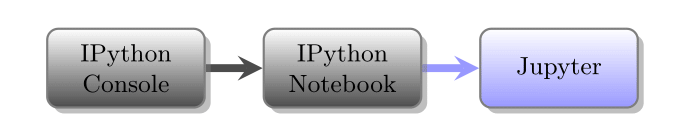
\includegraphics{images/diag-1.png}
\caption{Jupyter process}
\end{figure}

    \section{Le projet jupyter}\label{le-projet-jupyter}

Depuis la version 4, le projet ipython à été divsé en :

\begin{itemize}
\tightlist
\item
  \textbf{Jupyter(notebook, console, qtconsole)} - les interfaces
\item
  \textbf{ipython(ipykernel)} - le backend python
\item
  \textbf{ipywidgets} - éléments d'interfaces utilsateurs
\item
  \textbf{ipyparalléle} - framework d'exécution paralléle
\item
  \textbf{traitlets} - système de conf commun
\end{itemize}

    \section{Architecture de Jupyter}\label{architecture-de-jupyter}

\begin{figure}
\centering
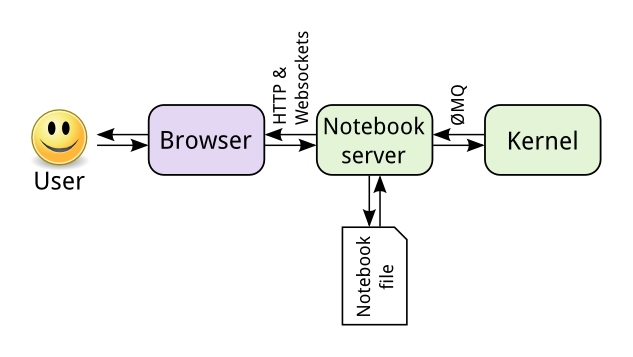
\includegraphics{images/notebook_components.png}
\caption{Jupyter process}
\end{figure}

    \section{IPython Architecture}\label{ipython-architecture}

\begin{figure}
\centering
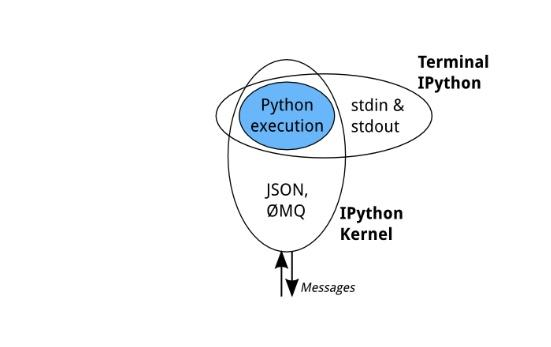
\includegraphics{images/building_custom_kernels_for_ipython.jpg}
\caption{Jupyter process}
\end{figure}

    \subsection{Des langages à volonté}\label{des-langages-uxe0-volontuxe9}

IPython Kernel supporte plus de 50 langage de programmation utiliser et
mélanger dans une même interface: Python, R, JavaScript, Ruby, Perl, C,
Julia, Fortran, Matlab ou Mathematica, SQLite et SQL.

https://github.com/jupyter/jupyter/wiki/Jupyter-kernels

    \subsection{Interfaces}\label{interfaces}

A premiére vue, le shell IPython et la console Jupyter sont identiques,
ils ont les memes fonctionalités utilisateurs lancer: - \$ ipython
console - \$ jupyter console

    Cependant, la commande jupyter console:

\begin{itemize}
\tightlist
\item
  lance deux processus: le noyau IPython + la console Jupyter(défaut)
\item
  ou permet de se connecter à un noyau existant, eventuellement
  distant(via ssh ou direct)
\end{itemize}

plusieurs consoles Jupyter peuvent partager le meme noyau

    En lançant la commande ipython on travaille directement avec IPython,
via stdin, stdout et stderr.

Outre l'économie de ressources, cela permet de l'utiliser comme un shell
système

    \section{Services IPython}\label{services-ipython}

En mode console, on à accès à toutes les fonctionnalités du noyau
IPython , à l'exception de l'affichage graphique riche des objets qui
n'est exploitable qu'avec le Notebook(et dans une moindre mesure avec
jupyter qtconsole)

    \subsubsection{Jupyter Console vs IPython
console}\label{jupyter-console-vs-ipython-console}

\begin{figure}
\centering
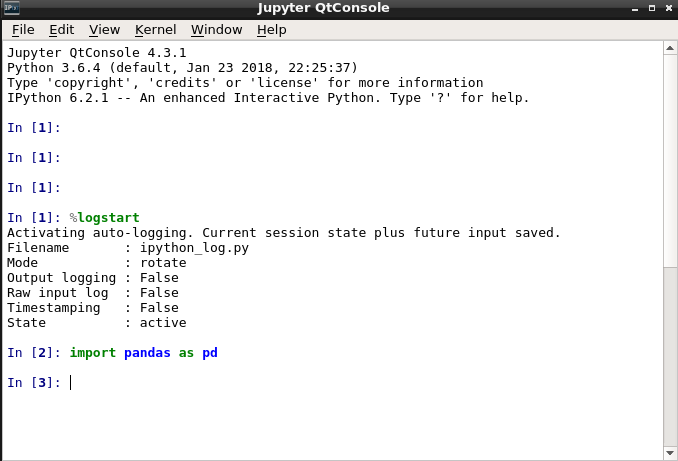
\includegraphics{images/jupyterqtconsole.png}
\caption{JupyterLab QtConsole}
\end{figure}

A premiére vue, le shell IPython et la console Jupyter sont identiques,
ils ont les memes fonctionnalités utilisateur.

    \textbf{\emph{Avec le notebook du Jupyter on a :}} - accés à tous les
services noyau de IPython y compris l'affichage riche des objets - la
possibilité d'inserer du texte formaté en markdown ou en LaTeX Le
document ainsi crée est enrgesitré au format .ipynb qui est du json -
les commandes magics commence avec (\%\%)dans la cellule notebook

Le document ainsi crée est enregistré au format .ipynb qui est au format
JSON.

    \subsection{Démarrage et organisation de
l'interface}\label{duxe9marrage-et-organisation-de-linterface}

** Démonstration ** - lancement du serveur; - présentation de
l'interface home; - ouverture et création d'un notebook; - changer le
titre; - notion de cellule et markdown; - illustration complétation et
documentation du notebook; - purger les sorties; - déplacer les
cellules; - racourcis clavier.

    \subsection{Le format .ipynb}\label{le-format-.ipynb}

\begin{figure}
\centering
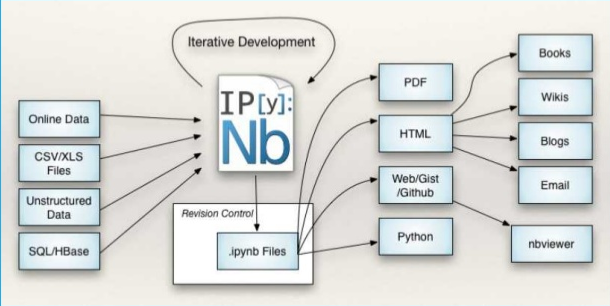
\includegraphics{images/IPython_Notebook_Workflows.png}
\caption{format}
\end{figure}

    \subsection{Lancement de Jupyter notebook en ligne de
commande}\label{lancement-de-jupyter-notebook-en-ligne-de-commande}

\begin{figure}
\centering
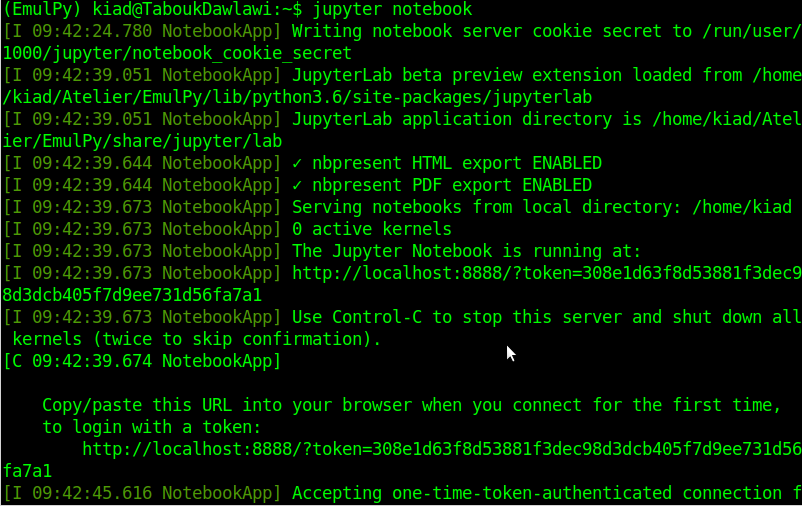
\includegraphics{images/jupyternotebook_run.png}
\caption{Jupyter process}
\end{figure}

    \subsection{Réprésentation integration des objets
riches}\label{ruxe9pruxe9sentation-integration-des-objets-riches}

IPython offre la possiblité aux objets Python de définir des
représentations autres que le simple

texte implementant des alternatives \_\emph{repr\_} (représentation d'un
objet en mode ascii):

\begin{itemize}
\tightlist
\item
  HTML (\emph{repr\_html})
\item
  JSON (\emph{repr\_json})
\item
  PNG (\emph{repr\_png})
\item
  JPEG (\emph{repr\_jpeg})
\item
  SVG (\emph{repr\_svg})
\item
  LaTeX (\emph{repr\_latex})
\end{itemize}

    \begin{Verbatim}[commandchars=\\\{\}]
{\color{incolor}In [{\color{incolor}4}]:} \PY{c+c1}{\PYZsh{}Utilisation d\PYZsq{}objet Python pour l\PYZsq{}affichage}
        \PY{k+kn}{from} \PY{n+nn}{IPython}\PY{n+nn}{.}\PY{n+nn}{display} \PY{k}{import} \PY{n}{Image}
        \PY{n}{img} \PY{o}{=} \PY{n}{Image}\PY{p}{(}\PY{l+s+s2}{\PYZdq{}}\PY{l+s+s2}{images/logo\PYZus{}collage.png}\PY{l+s+s2}{\PYZdq{}}\PY{p}{)}
        \PY{n}{img}
\end{Verbatim}

\texttt{\color{outcolor}Out[{\color{outcolor}4}]:}
    
    \begin{center}
    \adjustimage{max size={0.9\linewidth}{0.9\paperheight}}{output_40_0.png}
    \end{center}
    { \hspace*{\fill} \\}
    

    \begin{Verbatim}[commandchars=\\\{\}]
{\color{incolor}In [{\color{incolor}12}]:} \PY{n+nb}{print}\PY{p}{(}\PY{n}{img}\PY{o}{.}\PY{n}{\PYZus{}repr\PYZus{}png\PYZus{}}\PY{p}{(}\PY{p}{)}\PY{p}{[}\PY{p}{:}\PY{l+m+mi}{100}\PY{p}{]}\PY{p}{)}
\end{Verbatim}


    \begin{Verbatim}[commandchars=\\\{\}]
iVBORw0KGgoAAAANSUhEUgAABVYAAACaCAYAAABCKxN6AAFJ10lEQVR42uy9h1MUXRfue/6Fc2/dc2/dqlNffg1gzjkCEkRRQcRA

    \end{Verbatim}

    \begin{Verbatim}[commandchars=\\\{\}]
{\color{incolor}In [{\color{incolor}46}]:} \PY{k+kn}{from} \PY{n+nn}{IPython}\PY{n+nn}{.}\PY{n+nn}{display} \PY{k}{import} \PY{n}{Audio}
         \PY{n}{song} \PY{o}{=} \PY{n}{Audio}\PY{p}{(}\PY{l+s+s2}{\PYZdq{}}\PY{l+s+s2}{./data/001\PYZus{}Debutant\PYZus{}CD1.mp3}\PY{l+s+s2}{\PYZdq{}}\PY{p}{)}
         \PY{n}{song}
\end{Verbatim}


\begin{Verbatim}[commandchars=\\\{\}]
{\color{outcolor}Out[{\color{outcolor}46}]:} <IPython.lib.display.Audio object>
\end{Verbatim}
            
    \begin{Verbatim}[commandchars=\\\{\}]
{\color{incolor}In [{\color{incolor}47}]:} \PY{n+nb}{print}\PY{p}{(}\PY{n}{song}\PY{o}{.}\PY{n}{\PYZus{}repr\PYZus{}html\PYZus{}}\PY{p}{(}\PY{p}{)}\PY{p}{[}\PY{p}{:}\PY{l+m+mi}{200}\PY{p}{]}\PY{p}{)}
\end{Verbatim}


    \begin{Verbatim}[commandchars=\\\{\}]

                <audio controls="controls" >
                    <source src="data:audio/mpeg;base64,SUQzAwAAAAAhdlRQRTIAAAAOAAAATWljaGVsIFRob21hc1RZRVIAAAAFAAAAMjAwN1RSQ0sAAAADAAAAMDFUUFVCAAAAHgAAAE

    \end{Verbatim}

    \begin{Verbatim}[commandchars=\\\{\}]
{\color{incolor}In [{\color{incolor}48}]:} \PY{k+kn}{from} \PY{n+nn}{IPython}\PY{n+nn}{.}\PY{n+nn}{display} \PY{k}{import} \PY{n}{YouTubeVideo}
         \PY{n}{YouTubeVideo}\PY{p}{(}\PY{l+s+s2}{\PYZdq{}}\PY{l+s+s2}{8uWRVh58KdQ}\PY{l+s+s2}{\PYZdq{}}\PY{p}{)}
\end{Verbatim}

\texttt{\color{outcolor}Out[{\color{outcolor}48}]:}
    
    \begin{center}
    \adjustimage{max size={0.9\linewidth}{0.9\paperheight}}{output_44_0.jpeg}
    \end{center}
    { \hspace*{\fill} \\}
    

    \begin{Verbatim}[commandchars=\\\{\}]
{\color{incolor}In [{\color{incolor}49}]:} \PY{o}{\PYZpc{}}\PY{k}{matplotlib} inline
         
         \PY{k+kn}{import} \PY{n+nn}{numpy} \PY{k}{as} \PY{n+nn}{np}
         \PY{k+kn}{import} \PY{n+nn}{matplotlib}\PY{n+nn}{.}\PY{n+nn}{pyplot} \PY{k}{as} \PY{n+nn}{plt}
          
         \PY{n}{x} \PY{o}{=} \PY{n}{np}\PY{o}{.}\PY{n}{linspace}\PY{p}{(}\PY{l+m+mf}{0.1}\PY{p}{,} \PY{l+m+mi}{20}\PY{p}{,} \PY{l+m+mi}{200}\PY{p}{)}
         \PY{n}{fig}\PY{p}{,} \PY{n}{axe} \PY{o}{=} \PY{n}{plt}\PY{o}{.}\PY{n}{subplots}\PY{p}{(}\PY{n}{figsize}\PY{o}{=}\PY{p}{(}\PY{l+m+mi}{12}\PY{p}{,} \PY{l+m+mi}{8}\PY{p}{)}\PY{p}{)}
         \PY{n}{axe}\PY{o}{.}\PY{n}{plot}\PY{p}{(}\PY{n}{x}\PY{p}{,} \PY{n}{np}\PY{o}{.}\PY{n}{sin}\PY{p}{(}\PY{n}{x}\PY{p}{)}\PY{o}{/}\PY{n}{x}\PY{p}{)}
\end{Verbatim}


\begin{Verbatim}[commandchars=\\\{\}]
{\color{outcolor}Out[{\color{outcolor}49}]:} [<matplotlib.lines.Line2D at 0x7f2c2e3ec470>]
\end{Verbatim}
            
    \begin{center}
    \adjustimage{max size={0.9\linewidth}{0.9\paperheight}}{output_45_1.png}
    \end{center}
    { \hspace*{\fill} \\}
    
    \begin{Verbatim}[commandchars=\\\{\}]
{\color{incolor}In [{\color{incolor}50}]:} \PY{o}{\PYZpc{}}\PY{k}{matplotlib} notebook
         \PY{n}{fig}\PY{p}{,} \PY{n}{axe} \PY{o}{=} \PY{n}{plt}\PY{o}{.}\PY{n}{subplots}\PY{p}{(}\PY{n}{figsize}\PY{o}{=}\PY{p}{(}\PY{l+m+mi}{12}\PY{p}{,} \PY{l+m+mi}{8}\PY{p}{)}\PY{p}{)}
         \PY{n}{axe}\PY{o}{.}\PY{n}{plot}\PY{p}{(}\PY{n}{x}\PY{p}{,} \PY{n}{np}\PY{o}{.}\PY{n}{sin}\PY{p}{(}\PY{n}{x}\PY{p}{)}\PY{o}{/}\PY{n}{x}\PY{p}{)}
\end{Verbatim}


    
    \begin{verbatim}
<IPython.core.display.Javascript object>
    \end{verbatim}

    
    
    \begin{verbatim}
<IPython.core.display.HTML object>
    \end{verbatim}

    
\begin{Verbatim}[commandchars=\\\{\}]
{\color{outcolor}Out[{\color{outcolor}50}]:} [<matplotlib.lines.Line2D at 0x7f2c2bb71240>]
\end{Verbatim}
            
    
    \begin{verbatim}
<IPython.core.display.Javascript object>
    \end{verbatim}

    
    
    \begin{verbatim}
<IPython.core.display.HTML object>
    \end{verbatim}

    
    \subsection{Analyse de donnée:
Pandas}\label{analyse-de-donnuxe9e-pandas}

l'utilisation de la librairie Pandas rend la lecture de certains
formats, le regroupement de données et quelques traitements statistiques
trés simples.

    \begin{Verbatim}[commandchars=\\\{\}]
{\color{incolor}In [{\color{incolor}53}]:} \PY{k+kn}{import} \PY{n+nn}{pandas} \PY{k}{as} \PY{n+nn}{pd}
         \PY{k+kn}{import} \PY{n+nn}{numpy} \PY{k}{as} \PY{n+nn}{np}
         \PY{k+kn}{import} \PY{n+nn}{matplotlib}\PY{n+nn}{.}\PY{n+nn}{pyplot} \PY{k}{as} \PY{n+nn}{plt}
         \PY{n}{df} \PY{o}{=} \PY{n}{pd}\PY{o}{.}\PY{n}{read\PYZus{}excel}\PY{p}{(}\PY{l+s+s1}{\PYZsq{}}\PY{l+s+s1}{data/stock.xlsx}\PY{l+s+s1}{\PYZsq{}}\PY{p}{)}
         \PY{n}{df}\PY{o}{.}\PY{n}{dtypes}
\end{Verbatim}


\begin{Verbatim}[commandchars=\\\{\}]
{\color{outcolor}Out[{\color{outcolor}53}]:} VIN              object
         NUM ORDRE       float64
         CODE             object
         MODEL            object
         ETAT             object
         ARRIVAGE         object
         LOCALISATION     object
         COULEUR          object
         dtype: object
\end{Verbatim}
            
    \begin{Verbatim}[commandchars=\\\{\}]
{\color{incolor}In [{\color{incolor}54}]:} \PY{n}{df}\PY{o}{.}\PY{n}{info}\PY{p}{(}\PY{p}{)}
\end{Verbatim}


    \begin{Verbatim}[commandchars=\\\{\}]
<class 'pandas.core.frame.DataFrame'>
Int64Index: 113 entries, 1 to 113
Data columns (total 8 columns):
VIN             39 non-null object
NUM ORDRE       112 non-null float64
CODE            113 non-null object
MODEL           113 non-null object
ETAT            108 non-null object
ARRIVAGE        25 non-null object
LOCALISATION    18 non-null object
COULEUR         110 non-null object
dtypes: float64(1), object(7)
memory usage: 7.9+ KB

    \end{Verbatim}

    \subsection{Pandas charger un fichier
csv}\label{pandas-charger-un-fichier-csv}

\url{https://github.com/shantnu/Intro-to-Pandas}

    \begin{Verbatim}[commandchars=\\\{\}]
{\color{incolor}In [{\color{incolor}55}]:} \PY{o}{\PYZpc{}}\PY{k}{matplotlib} inline
         \PY{n}{data} \PY{o}{=} \PY{n}{pd}\PY{o}{.}\PY{n}{read\PYZus{}csv}\PY{p}{(}\PY{l+s+s2}{\PYZdq{}}\PY{l+s+s2}{./example/hubble\PYZus{}data.csv}\PY{l+s+s2}{\PYZdq{}}\PY{p}{)}
         \PY{n}{data}\PY{o}{.}\PY{n}{head}\PY{p}{(}\PY{p}{)}
\end{Verbatim}


\begin{Verbatim}[commandchars=\\\{\}]
{\color{outcolor}Out[{\color{outcolor}55}]:}    distance  recession\_velocity
         0     0.032                 170
         1     0.034                 290
         2     0.214                -130
         3     0.263                 -70
         4     0.275                -185
\end{Verbatim}
            
    \begin{Verbatim}[commandchars=\\\{\}]
{\color{incolor}In [{\color{incolor}56}]:} \PY{n}{data}\PY{o}{.}\PY{n}{info}\PY{p}{(}\PY{p}{)}
\end{Verbatim}


    \begin{Verbatim}[commandchars=\\\{\}]
<class 'pandas.core.frame.DataFrame'>
RangeIndex: 24 entries, 0 to 23
Data columns (total 2 columns):
distance              24 non-null float64
recession\_velocity    24 non-null int64
dtypes: float64(1), int64(1)
memory usage: 464.0 bytes

    \end{Verbatim}

    \begin{Verbatim}[commandchars=\\\{\}]
{\color{incolor}In [{\color{incolor}57}]:} \PY{n}{headers} \PY{o}{=} \PY{p}{[}\PY{l+s+s2}{\PYZdq{}}\PY{l+s+s2}{dist}\PY{l+s+s2}{\PYZdq{}}\PY{p}{,}\PY{l+s+s2}{\PYZdq{}}\PY{l+s+s2}{rec\PYZus{}vel}\PY{l+s+s2}{\PYZdq{}}\PY{p}{]}
         \PY{n}{data\PYZus{}no\PYZus{}headers} \PY{o}{=} \PY{n}{pd}\PY{o}{.}\PY{n}{read\PYZus{}csv}\PY{p}{(}\PY{l+s+s2}{\PYZdq{}}\PY{l+s+s2}{./example/hubble\PYZus{}data\PYZus{}no\PYZus{}headers.csv}\PY{l+s+s2}{\PYZdq{}}\PY{p}{,} \PY{n}{names} \PY{o}{=} \PY{n}{headers}\PY{p}{)}
         \PY{n}{data\PYZus{}no\PYZus{}headers}\PY{o}{.}\PY{n}{head}\PY{p}{(}\PY{p}{)}
\end{Verbatim}


\begin{Verbatim}[commandchars=\\\{\}]
{\color{outcolor}Out[{\color{outcolor}57}]:}     dist  rec\_vel
         0  0.032      170
         1  0.034      290
         2  0.214     -130
         3  0.263      -70
         4  0.275     -185
\end{Verbatim}
            
    \textbf{Selectionné d'une colonne}

    \begin{Verbatim}[commandchars=\\\{\}]
{\color{incolor}In [{\color{incolor}59}]:} \PY{n}{data\PYZus{}no\PYZus{}headers}\PY{p}{[}\PY{l+s+s2}{\PYZdq{}}\PY{l+s+s2}{dist}\PY{l+s+s2}{\PYZdq{}}\PY{p}{]}\PY{o}{.}\PY{n}{tail}\PY{p}{(}\PY{l+m+mi}{4}\PY{p}{)}
\end{Verbatim}


\begin{Verbatim}[commandchars=\\\{\}]
{\color{outcolor}Out[{\color{outcolor}59}]:} 20    2.0
         21    2.0
         22    2.0
         23    2.0
         Name: dist, dtype: float64
\end{Verbatim}
            
    \textbf{\emph{Jouer avec les index}}

    \begin{Verbatim}[commandchars=\\\{\}]
{\color{incolor}In [{\color{incolor}60}]:} \PY{n}{data}\PY{o}{.}\PY{n}{set\PYZus{}index}\PY{p}{(}\PY{l+s+s2}{\PYZdq{}}\PY{l+s+s2}{distance}\PY{l+s+s2}{\PYZdq{}}\PY{p}{,} \PY{n}{inplace}\PY{o}{=} \PY{k+kc}{True}\PY{p}{)}
         \PY{n}{data}\PY{o}{.}\PY{n}{head}\PY{p}{(}\PY{p}{)}
\end{Verbatim}


\begin{Verbatim}[commandchars=\\\{\}]
{\color{outcolor}Out[{\color{outcolor}60}]:}           recession\_velocity
         distance                    
         0.032                    170
         0.034                    290
         0.214                   -130
         0.263                    -70
         0.275                   -185
\end{Verbatim}
            
    \begin{Verbatim}[commandchars=\\\{\}]
{\color{incolor}In [{\color{incolor}61}]:} \PY{n}{data}\PY{o}{.}\PY{n}{plot}\PY{p}{(}\PY{p}{)}
         \PY{n}{plt}\PY{o}{.}\PY{n}{show}\PY{p}{(}\PY{p}{)}
\end{Verbatim}


    \begin{center}
    \adjustimage{max size={0.9\linewidth}{0.9\paperheight}}{output_58_0.png}
    \end{center}
    { \hspace*{\fill} \\}
    
    \subsection{Un autre exemple}\label{un-autre-exemple}

    \begin{Verbatim}[commandchars=\\\{\}]
{\color{incolor}In [{\color{incolor}62}]:} \PY{n}{data} \PY{o}{=} \PY{n}{pd}\PY{o}{.}\PY{n}{read\PYZus{}csv}\PY{p}{(}\PY{l+s+s2}{\PYZdq{}}\PY{l+s+s2}{./example/wages\PYZus{}hours.csv}\PY{l+s+s2}{\PYZdq{}}\PY{p}{)}
         \PY{n}{data}\PY{o}{.}\PY{n}{head}\PY{p}{(}\PY{p}{)}
\end{Verbatim}


\begin{Verbatim}[commandchars=\\\{\}]
{\color{outcolor}Out[{\color{outcolor}62}]:}   HRS\textbackslash{}tRATE\textbackslash{}tERSP\textbackslash{}tERNO\textbackslash{}tNEIN\textbackslash{}tASSET\textbackslash{}tAGE\textbackslash{}tDEP\textbackslash{}tRACE\textbackslash{}tSCHOOL
         0  2157\textbackslash{}t2.905\textbackslash{}t1121\textbackslash{}t291\textbackslash{}t380\textbackslash{}t7250\textbackslash{}t38.5\textbackslash{}t2.340{\ldots}        
         1  2174\textbackslash{}t2.970\textbackslash{}t1128\textbackslash{}t301\textbackslash{}t398\textbackslash{}t7744\textbackslash{}t39.3\textbackslash{}t2.335{\ldots}        
         2  2062\textbackslash{}t2.350\textbackslash{}t1214\textbackslash{}t326\textbackslash{}t185\textbackslash{}t3068\textbackslash{}t40.1\textbackslash{}t2.851{\ldots}        
         3  2111\textbackslash{}t2.511\textbackslash{}t1203\textbackslash{}t49\textbackslash{}t117\textbackslash{}t1632\textbackslash{}t22.4\textbackslash{}t1.159\textbackslash{}{\ldots}        
         4  2134\textbackslash{}t2.791\textbackslash{}t1013\textbackslash{}t594\textbackslash{}t730\textbackslash{}t12710\textbackslash{}t57.7\textbackslash{}t1.22{\ldots}        
\end{Verbatim}
            
    \textbf{\emph{filter l'affichage}}

    \begin{Verbatim}[commandchars=\\\{\}]
{\color{incolor}In [{\color{incolor}63}]:} \PY{n}{data} \PY{o}{=} \PY{n}{pd}\PY{o}{.}\PY{n}{read\PYZus{}csv}\PY{p}{(}\PY{l+s+s2}{\PYZdq{}}\PY{l+s+s2}{./example/wages\PYZus{}hours.csv}\PY{l+s+s2}{\PYZdq{}}\PY{p}{,} \PY{n}{sep} \PY{o}{=} \PY{l+s+s2}{\PYZdq{}}\PY{l+s+se}{\PYZbs{}t}\PY{l+s+s2}{\PYZdq{}}\PY{p}{)}
         \PY{n}{data}\PY{o}{.}\PY{n}{head}\PY{p}{(}\PY{p}{)}
\end{Verbatim}


\begin{Verbatim}[commandchars=\\\{\}]
{\color{outcolor}Out[{\color{outcolor}63}]:}     HRS   RATE  ERSP ERNO  NEIN  ASSET   AGE    DEP  RACE  SCHOOL
         0  2157  2.905  1121  291   380   7250  38.5  2.340  32.1    10.5
         1  2174  2.970  1128  301   398   7744  39.3  2.335  31.2    10.5
         2  2062  2.350  1214  326   185   3068  40.1  2.851     *     8.9
         3  2111  2.511  1203   49   117   1632  22.4  1.159  27.5    11.5
         4  2134  2.791  1013  594   730  12710  57.7  1.229  32.5     8.8
\end{Verbatim}
            
    \textbf{\emph{l'âge par rapport au taux (salaire)}}

    \begin{Verbatim}[commandchars=\\\{\}]
{\color{incolor}In [{\color{incolor}20}]:} \PY{n}{data2} \PY{o}{=} \PY{n}{data}\PY{p}{[}\PY{p}{[}\PY{l+s+s2}{\PYZdq{}}\PY{l+s+s2}{AGE}\PY{l+s+s2}{\PYZdq{}}\PY{p}{,} \PY{l+s+s2}{\PYZdq{}}\PY{l+s+s2}{RATE}\PY{l+s+s2}{\PYZdq{}}\PY{p}{]}\PY{p}{]}
         \PY{n}{data2}\PY{o}{.}\PY{n}{head}\PY{p}{(}\PY{p}{)}
\end{Verbatim}


\begin{Verbatim}[commandchars=\\\{\}]
{\color{outcolor}Out[{\color{outcolor}20}]:}     AGE   RATE
         0  38.5  2.905
         1  39.3  2.970
         2  40.1  2.350
         3  22.4  2.511
         4  57.7  2.791
\end{Verbatim}
            
    \textbf{\emph{trier par valeur}}

    \begin{Verbatim}[commandchars=\\\{\}]
{\color{incolor}In [{\color{incolor}22}]:} \PY{n}{data\PYZus{}sorted} \PY{o}{=} \PY{n}{data2}\PY{o}{.}\PY{n}{sort\PYZus{}values}\PY{p}{(}\PY{p}{[}\PY{l+s+s2}{\PYZdq{}}\PY{l+s+s2}{AGE}\PY{l+s+s2}{\PYZdq{}}\PY{p}{]}\PY{p}{)}
         \PY{n}{data\PYZus{}sorted}\PY{o}{.}\PY{n}{head}\PY{p}{(}\PY{p}{)}
\end{Verbatim}


\begin{Verbatim}[commandchars=\\\{\}]
{\color{outcolor}Out[{\color{outcolor}22}]:}      AGE   RATE
         3   22.4  2.511
         27  37.2  3.015
         31  37.4  1.901
         33  37.5  1.899
         32  37.5  3.009
\end{Verbatim}
            
    \textbf{\emph{trier par index}}

    \begin{Verbatim}[commandchars=\\\{\}]
{\color{incolor}In [{\color{incolor}64}]:} \PY{n}{data\PYZus{}sorted}\PY{o}{.}\PY{n}{set\PYZus{}index}\PY{p}{(}\PY{l+s+s2}{\PYZdq{}}\PY{l+s+s2}{AGE}\PY{l+s+s2}{\PYZdq{}}\PY{p}{,} \PY{n}{inplace}\PY{o}{=}\PY{k+kc}{True}\PY{p}{)}
         \PY{n}{data\PYZus{}sorted}\PY{o}{.}\PY{n}{head}\PY{p}{(}\PY{p}{)}
\end{Verbatim}


    \begin{Verbatim}[commandchars=\\\{\}]

        ---------------------------------------------------------------------------

        KeyError                                  Traceback (most recent call last)

        \textasciitilde{}/Atelier/EmulPy/lib/python3.6/site-packages/pandas/core/indexes/base.py in get\_loc(self, key, method, tolerance)
       2524             try:
    -> 2525                 return self.\_engine.get\_loc(key)
       2526             except KeyError:


        pandas/\_libs/index.pyx in pandas.\_libs.index.IndexEngine.get\_loc()


        pandas/\_libs/index.pyx in pandas.\_libs.index.IndexEngine.get\_loc()


        pandas/\_libs/hashtable\_class\_helper.pxi in pandas.\_libs.hashtable.PyObjectHashTable.get\_item()


        pandas/\_libs/hashtable\_class\_helper.pxi in pandas.\_libs.hashtable.PyObjectHashTable.get\_item()


        KeyError: 'AGE'

        
    During handling of the above exception, another exception occurred:


        KeyError                                  Traceback (most recent call last)

        <ipython-input-64-131969dddbae> in <module>()
    ----> 1 data\_sorted.set\_index("AGE", inplace=True)
          2 data\_sorted.head()


        \textasciitilde{}/Atelier/EmulPy/lib/python3.6/site-packages/pandas/core/frame.py in set\_index(self, keys, drop, append, inplace, verify\_integrity)
       3144                 names.append(None)
       3145             else:
    -> 3146                 level = frame[col].\_values
       3147                 names.append(col)
       3148                 if drop:


        \textasciitilde{}/Atelier/EmulPy/lib/python3.6/site-packages/pandas/core/frame.py in \_\_getitem\_\_(self, key)
       2137             return self.\_getitem\_multilevel(key)
       2138         else:
    -> 2139             return self.\_getitem\_column(key)
       2140 
       2141     def \_getitem\_column(self, key):


        \textasciitilde{}/Atelier/EmulPy/lib/python3.6/site-packages/pandas/core/frame.py in \_getitem\_column(self, key)
       2144         \# get column
       2145         if self.columns.is\_unique:
    -> 2146             return self.\_get\_item\_cache(key)
       2147 
       2148         \# duplicate columns \& possible reduce dimensionality


        \textasciitilde{}/Atelier/EmulPy/lib/python3.6/site-packages/pandas/core/generic.py in \_get\_item\_cache(self, item)
       1840         res = cache.get(item)
       1841         if res is None:
    -> 1842             values = self.\_data.get(item)
       1843             res = self.\_box\_item\_values(item, values)
       1844             cache[item] = res


        \textasciitilde{}/Atelier/EmulPy/lib/python3.6/site-packages/pandas/core/internals.py in get(self, item, fastpath)
       3841 
       3842             if not isna(item):
    -> 3843                 loc = self.items.get\_loc(item)
       3844             else:
       3845                 indexer = np.arange(len(self.items))[isna(self.items)]


        \textasciitilde{}/Atelier/EmulPy/lib/python3.6/site-packages/pandas/core/indexes/base.py in get\_loc(self, key, method, tolerance)
       2525                 return self.\_engine.get\_loc(key)
       2526             except KeyError:
    -> 2527                 return self.\_engine.get\_loc(self.\_maybe\_cast\_indexer(key))
       2528 
       2529         indexer = self.get\_indexer([key], method=method, tolerance=tolerance)


        pandas/\_libs/index.pyx in pandas.\_libs.index.IndexEngine.get\_loc()


        pandas/\_libs/index.pyx in pandas.\_libs.index.IndexEngine.get\_loc()


        pandas/\_libs/hashtable\_class\_helper.pxi in pandas.\_libs.hashtable.PyObjectHashTable.get\_item()


        pandas/\_libs/hashtable\_class\_helper.pxi in pandas.\_libs.hashtable.PyObjectHashTable.get\_item()


        KeyError: 'AGE'

    \end{Verbatim}

    \textbf{\emph{le taux augmente jusqu'à l'âge de 35 ans, puis il varie
considérablement.}}

    \begin{Verbatim}[commandchars=\\\{\}]
{\color{incolor}In [{\color{incolor}24}]:} \PY{n}{data\PYZus{}sorted}\PY{o}{.}\PY{n}{plot}\PY{p}{(}\PY{p}{)}
         \PY{n}{plt}\PY{o}{.}\PY{n}{show}\PY{p}{(}\PY{p}{)}
\end{Verbatim}


    \begin{center}
    \adjustimage{max size={0.9\linewidth}{0.9\paperheight}}{output_70_0.png}
    \end{center}
    { \hspace*{\fill} \\}
    
    \subsection{Calcul formel}\label{calcul-formel}

    \begin{Verbatim}[commandchars=\\\{\}]
{\color{incolor}In [{\color{incolor}35}]:} \PY{k+kn}{from} \PY{n+nn}{sympy} \PY{k}{import} \PY{o}{*}
         \PY{c+c1}{\PYZsh{} Initialize notebook printing}
         \PY{n}{init\PYZus{}printing}\PY{p}{(}\PY{p}{)}
         \PY{n}{integrate}\PY{p}{(}\PY{n}{x}\PY{o}{*}\PY{o}{*}\PY{l+m+mi}{2} \PY{o}{*} \PY{n}{exp}\PY{p}{(}\PY{n}{x}\PY{p}{)} \PY{o}{*} \PY{n}{cos}\PY{p}{(}\PY{n}{x}\PY{p}{)}\PY{p}{,} \PY{n}{x}\PY{p}{)}
\end{Verbatim}

\texttt{\color{outcolor}Out[{\color{outcolor}35}]:}
    
    $$\frac{x^{2} e^{x}}{2} \sin{\left (x \right )} + \frac{x^{2} e^{x}}{2} \cos{\left (x \right )} - x e^{x} \sin{\left (x \right )} + \frac{e^{x}}{2} \sin{\left (x \right )} - \frac{e^{x}}{2} \cos{\left (x \right )}$$

    

    \begin{Verbatim}[commandchars=\\\{\}]
{\color{incolor}In [{\color{incolor}36}]:} \PY{k+kn}{from} \PY{n+nn}{sympy}\PY{n+nn}{.}\PY{n+nn}{integrals} \PY{k}{import} \PY{n}{laplace\PYZus{}transform}
         \PY{k+kn}{from} \PY{n+nn}{sympy}\PY{n+nn}{.}\PY{n+nn}{abc} \PY{k}{import} \PY{n}{t}\PY{p}{,} \PY{n}{s}\PY{p}{,} \PY{n}{a}
         \PY{n}{laplace\PYZus{}transform}\PY{p}{(}\PY{n}{t}\PY{o}{*}\PY{o}{*}\PY{n}{a}\PY{p}{,} \PY{n}{t}\PY{p}{,} \PY{n}{s}\PY{p}{)}
\end{Verbatim}

\texttt{\color{outcolor}Out[{\color{outcolor}36}]:}
    
    $$\left ( \frac{s^{- a}}{s} \Gamma{\left(a + 1 \right)}, \quad 0, \quad - \Re{\left(a\right)} < 1\right )$$

    

    \subsection{Cellules de texte riche}\label{cellules-de-texte-riche}

Dans ces cellules on peut saisir du texte aves des balises de lise en
forme:

\begin{itemize}
\tightlist
\item
  Markdown
\item
  HTML
\item
  LaTeX
\end{itemize}

    \subsubsection{Démo (Texte Markdown)}\label{duxe9mo-texte-markdown}

    \subsubsection{IPywidgets}\label{ipywidgets}

Une extension IPython pour ajouter encore plus d'interactivité à nos
Notebooks.

    \subsubsection{IPywidgets}\label{ipywidgets}

Les IPywidgets sont des éléments graphiques permettant de piloter des
paramétres de fonctions - des zones de saisies - des cases à cocher -
des curseurs - des menus déroulants

    La clé réside dans la commande interact

    \begin{Verbatim}[commandchars=\\\{\}]
{\color{incolor}In [{\color{incolor}67}]:} \PY{k+kn}{from} \PY{n+nn}{ipywidgets} \PY{k}{import} \PY{n}{interact}
\end{Verbatim}


    \subsubsection{Premier exemple}\label{premier-exemple}

    \begin{Verbatim}[commandchars=\\\{\}]
{\color{incolor}In [{\color{incolor}66}]:} \PY{k+kn}{from} \PY{n+nn}{ipywidgets} \PY{k}{import} \PY{o}{*}
         \PY{k+kn}{from} \PY{n+nn}{IPython}\PY{n+nn}{.}\PY{n+nn}{display} \PY{k}{import} \PY{n}{display}
         \PY{n}{w} \PY{o}{=} \PY{n}{IntSlider}\PY{p}{(}\PY{p}{)}
         \PY{n}{display}\PY{p}{(}\PY{n}{w}\PY{p}{,} \PY{n}{w}\PY{p}{)}
\end{Verbatim}


    
    \begin{verbatim}
IntSlider(value=0)
    \end{verbatim}

    
    
    \begin{verbatim}
IntSlider(value=0)
    \end{verbatim}

    
    \subsubsection{Deuxième exemple}\label{deuxiuxe8me-exemple}

    \begin{Verbatim}[commandchars=\\\{\}]
{\color{incolor}In [{\color{incolor}68}]:} \PY{k}{def} \PY{n+nf}{f}\PY{p}{(}\PY{n}{x}\PY{p}{)}\PY{p}{:}
             \PY{n+nb}{print}\PY{p}{(}\PY{n}{x}\PY{p}{)}
         \PY{n}{interact}\PY{p}{(}\PY{n}{f}\PY{p}{,} \PY{n}{x}\PY{o}{=}\PY{l+m+mi}{10}\PY{p}{)}
\end{Verbatim}


    
    \begin{verbatim}
interactive(children=(IntSlider(value=10, description='x', max=30, min=-10), Output()), _dom_classes=('widget-interact',))
    \end{verbatim}

    
\begin{Verbatim}[commandchars=\\\{\}]
{\color{outcolor}Out[{\color{outcolor}68}]:} <function \_\_main\_\_.f>
\end{Verbatim}
            
    \begin{Verbatim}[commandchars=\\\{\}]
{\color{incolor}In [{\color{incolor}69}]:} \PY{n}{interact}\PY{p}{(}\PY{n}{f}\PY{p}{,} \PY{n}{x}\PY{o}{=}\PY{k+kc}{True}\PY{p}{)} \PY{c+c1}{\PYZsh{}Or False}
\end{Verbatim}


    
    \begin{verbatim}
interactive(children=(Checkbox(value=True, description='x'), Output()), _dom_classes=('widget-interact',))
    \end{verbatim}

    
\begin{Verbatim}[commandchars=\\\{\}]
{\color{outcolor}Out[{\color{outcolor}69}]:} <function \_\_main\_\_.f>
\end{Verbatim}
            
    \textbf{\emph{valeur booléen}}

    \begin{Verbatim}[commandchars=\\\{\}]
{\color{incolor}In [{\color{incolor}70}]:} \PY{n}{interact}\PY{p}{(}\PY{n}{f}\PY{p}{,} \PY{n}{x}\PY{o}{=}\PY{l+s+s1}{\PYZsq{}}\PY{l+s+s1}{text}\PY{l+s+s1}{\PYZsq{}}\PY{p}{)}
\end{Verbatim}


    
    \begin{verbatim}
interactive(children=(Text(value='text', description='x'), Output()), _dom_classes=('widget-interact',))
    \end{verbatim}

    
\begin{Verbatim}[commandchars=\\\{\}]
{\color{outcolor}Out[{\color{outcolor}70}]:} <function \_\_main\_\_.f>
\end{Verbatim}
            
    \begin{Verbatim}[commandchars=\\\{\}]
{\color{incolor}In [{\color{incolor}71}]:} \PY{k+kn}{from} \PY{n+nn}{ipywidgets} \PY{k}{import} \PY{n}{interact}
         \PY{n}{t} \PY{o}{=} \PY{n}{np}\PY{o}{.}\PY{n}{arange}\PY{p}{(}\PY{l+m+mf}{0.0}\PY{p}{,} \PY{l+m+mf}{1.0}\PY{p}{,} \PY{l+m+mf}{0.01}\PY{p}{)}
         \PY{n}{x} \PY{o}{=} \PY{n}{np}\PY{o}{.}\PY{n}{linspace}\PY{p}{(}\PY{l+m+mi}{0}\PY{p}{,} \PY{l+m+mi}{2}\PY{o}{*}\PY{n}{np}\PY{o}{.}\PY{n}{pi}\PY{p}{,} \PY{l+m+mi}{100}\PY{p}{)}
         
         \PY{k}{def} \PY{n+nf}{pltsin}\PY{p}{(}\PY{n}{f}\PY{p}{)}\PY{p}{:}
             \PY{n}{plt}\PY{o}{.}\PY{n}{plot}\PY{p}{(}\PY{n}{x}\PY{p}{,} \PY{n}{sin}\PY{p}{(}\PY{l+m+mi}{2}\PY{o}{*}\PY{n}{np}\PY{o}{.}\PY{n}{pi}\PY{o}{*}\PY{n}{t}\PY{o}{*}\PY{n}{f}\PY{p}{)}\PY{p}{)}
             \PY{n}{plt}\PY{o}{.}\PY{n}{show}\PY{p}{(}\PY{p}{)}
         \PY{n}{interact}\PY{p}{(}\PY{n}{pltsin}\PY{p}{,} \PY{n}{f}\PY{o}{=}\PY{p}{(}\PY{l+m+mi}{1}\PY{p}{,} \PY{l+m+mi}{10}\PY{p}{,} \PY{l+m+mf}{0.1}\PY{p}{)}\PY{p}{)}
         \PY{n}{t}
\end{Verbatim}


    
    \begin{verbatim}
interactive(children=(FloatSlider(value=5.0, description='f', max=10.0, min=1.0), Output()), _dom_classes=('widget-interact',))
    \end{verbatim}

    
\begin{Verbatim}[commandchars=\\\{\}]
{\color{outcolor}Out[{\color{outcolor}71}]:} array([0.  , 0.01, 0.02, 0.03, 0.04, 0.05, 0.06, 0.07, 0.08, 0.09, 0.1 ,
                0.11, 0.12, 0.13, 0.14, 0.15, 0.16, 0.17, 0.18, 0.19, 0.2 , 0.21,
                0.22, 0.23, 0.24, 0.25, 0.26, 0.27, 0.28, 0.29, 0.3 , 0.31, 0.32,
                0.33, 0.34, 0.35, 0.36, 0.37, 0.38, 0.39, 0.4 , 0.41, 0.42, 0.43,
                0.44, 0.45, 0.46, 0.47, 0.48, 0.49, 0.5 , 0.51, 0.52, 0.53, 0.54,
                0.55, 0.56, 0.57, 0.58, 0.59, 0.6 , 0.61, 0.62, 0.63, 0.64, 0.65,
                0.66, 0.67, 0.68, 0.69, 0.7 , 0.71, 0.72, 0.73, 0.74, 0.75, 0.76,
                0.77, 0.78, 0.79, 0.8 , 0.81, 0.82, 0.83, 0.84, 0.85, 0.86, 0.87,
                0.88, 0.89, 0.9 , 0.91, 0.92, 0.93, 0.94, 0.95, 0.96, 0.97, 0.98,
                0.99])
\end{Verbatim}
            
    \$ pip install ipywidgets

\$ jupyter nbextension enable -\/-py -\/-sys-prefix widgetsnbextension

    \section{Un mot sur JupyterLab (l'environnement de développement
web)}\label{un-mot-sur-jupyterlab-lenvironnement-de-duxe9veloppement-web}

\begin{figure}
\centering
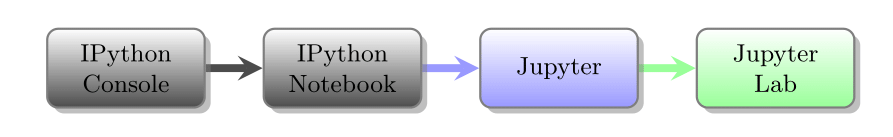
\includegraphics{images/diag-2.png}
\caption{JupyterLab process}
\end{figure}

    \subsubsection{Quelques différences avec
Jupyter}\label{quelques-diffuxe9rences-avec-jupyter}

\begin{itemize}
\tightlist
\item
  glisser-déposer pour réorganiser les cellules d'un notebook et les
  copier entre les notebooks.
\item
  l'affichage un moteur de rendu plus récent.
\item
  exécution des blocs de code de manière interactive à partir de
  fichiers texte (.py, .R, .md, .tex, etc.) ;
\item
  associer une console de code à un kernel de notebook pour explorer le
  code de manière interactive sans encombrer le notebook avec un travail
  temporaire ;
\item
  le tout en un, editeur JSON, console d'administration, composant web,
  notebooks un IDE scientifique intégéré avec une logique web
\item
  modifier les formats de fichiers populaires avec un aperçu en direct,
  tel que Markdown, JSON, CSV, Vega, VegaLite, et plus encore.
\end{itemize}

    \subsection{Démo}\label{duxe9mo}

    \subsubsection{Les extensions de
JupyterLab}\label{les-extensions-de-jupyterlab}

JupyterLab dispose d'une option pour liste les extensions:

\$ jupyterlab labextension list

Pour installer une extension pour jupyter

\$ jupyter labextension install jupyterlab\_voyager

jupyter labextension disable

jupyter labextension enable

https://jupyterlab.readthedocs.io/en/latest/developer/extension\_dev.html

    \subsubsection{Interagir avec le Kernel}\label{interagir-avec-le-kernel}

\$ jupyter kernelspec list

Available kernels:

bash /home/kiad/.local/share/jupyter/kernels/bash

python3 /home/kiad/.local/share/jupyter/kernels/python3

octave /home/kiad/Atelier/EmulPy/share/jupyter/kernels/

scilab /home/kiad/Atelier/EmulPy/share/jupyter/kernels/scilab

coarray-fortran /usr/local/share/jupyter/kernels/coarray-fortran

python2 /usr/share/jupyter/kernels/python2

sagemath /usr/share/jupyter/kernels/sagemath

    \section{Conversion et publication}\label{conversion-et-publication}

L'outil nbconvert est un outil en ligne de commandes qui permet de
convertir les fichiers .ipynb dans un des formats supportés: HTML, PDF
via LaTeX, diapositives(reveal.js), script, markdown, ReStructured Text.

\begin{quote}
jupyter nbconvert -\/-to pdf votre\_fichier.ipynb
\end{quote}

\begin{quote}
jupyter nbconvert -\/-to html -\/-template base votre\_fichier.ipynb
\end{quote}

\begin{quote}
jupyter nbconvert slides.ipynb -\/-to slides -\/-post serve
-\/-ServePostProcessor.reveal\_cdn="http://cdn.jsdelivr.net/reveal.js/2.5.0"
\end{quote}

    *** Démonstration *** - le notebook de cette présentation - les
méta-données de cellule.

    \subsection{nbviewer Publication sur internet (Un livre écrit totalement
avec
Jupyter)}\label{nbviewer-publication-sur-internet-un-livre-uxe9crit-totalement-avec-jupyter}

    \section{Coopération et partage}\label{coopuxe9ration-et-partage}

Avec d'autres utilisateurs de jupyter:

\begin{itemize}
\tightlist
\item
  On peut facilement partager le notebook lui meme

  \begin{itemize}
  \tightlist
  \item
    par email
  \item
    par répertoire partagé
  \item
    dans le cloud
  \item
    via un VCS privé ou github/bitbucket
  \end{itemize}
\item
  Ou utiliser JupyterHub (https://github.com/jupyterhub/jupyterhub) dans
  une origanisation
\end{itemize}

    \begin{Verbatim}[commandchars=\\\{\}]
{\color{incolor}In [{\color{incolor} }]:} \PY{c+c1}{\PYZsh{}  Questions?}
        
           
\end{Verbatim}



    % Add a bibliography block to the postdoc
    
    
    
    \end{document}
